%!TEX root = ../Thesis.tex

\section{Performance and robustness improving techniques}\label{sec: Theory: Performance and robustness improving techniques}

\subsection{Fitness rank transform}\label{sec: Theory: Performance and robustness improving techniques: Fitness rank transform}
\begin{figure}[tbp!]
    \begin{subfigure}[b]{0.485\textwidth}
        \centering
        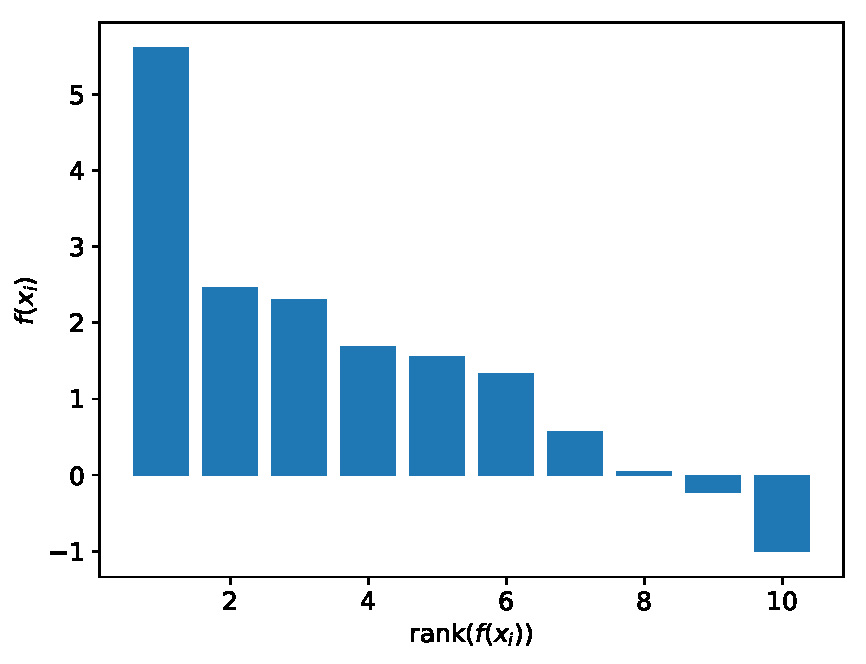
\includegraphics[height=5.8cm]{graphics/fitness-transform/fitnesses.pdf}
        \caption{}
        \label{fig: Theory: fitness-transform/fitnesses.pdf}
    \end{subfigure}
    \hfill
    \begin{subfigure}[b]{0.495\textwidth}
        \centering
        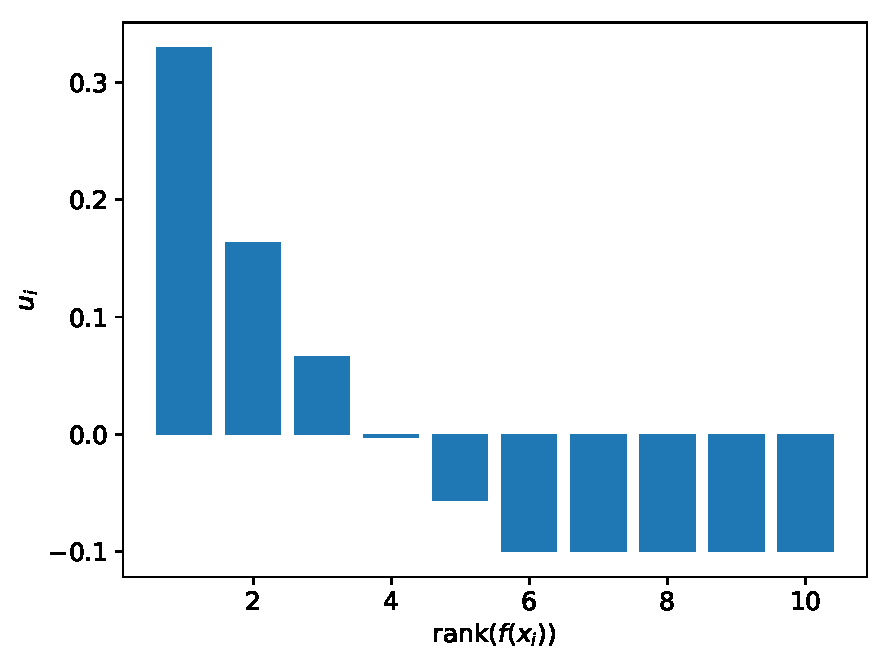
\includegraphics[height=5.8cm]{graphics/fitness-transform/transform.pdf}
        \caption{}
        \label{fig: Theory: fitness-transform/transform.pdf}
    \end{subfigure}
    \caption{
        Illustration of the fitness rank transform applied to evaluated fitnesses.
        \subref{fig: Theory: fitness-transform/fitnesses.pdf} Ten randomly sampled fitnesses. 
        \subref{fig: Theory: fitness-transform/transform.pdf} The ten corresponding utilities according to \eqref{eq: Theory: Fitness rank transform}.
    }
    \label{fig: Theory: fitness-transform}
\end{figure}
In general, the values returned by the function being optimized, $f(\x_i)$, may vary wildly in size depending on the function and the points at which it is sampled. Directly using the returned function value makes hyperparameters, such as the learning rate, highly dependent on the objective function. Additionally, the returned function values may increase or decrease considerably as the algorithm converges to an optimum. Clearly, this can result in numerical instability and hyperparameters being highly dependent on the objective function is undesirable.

One way to avoid this is to transform the function values before they are used to compute the gradient. One possible transform type is the so-called rank transform. 
This transform ranks the sampled function values $f(\x_i)$ and assigns to each one a value that depends only the relative value of the sample compared to the other samples. These new values are called utilities.
Utilities do not change in size during optimization and have no dependency on the actual value of the objective function but do encode information on the relative fitness of the samples. Replacing thge function values by utlities makes \gls{VO} invariant to any order-preserving transformation of the objective function such as addition or multiplication by a scalar \cite{Wierstra2008}. To decouple the learning rate of the algorithm from the utilities it is appropriate to require that $\sum_{i=1}^N \size{u_i} = C$ for some constant $C$.

Several possible choices of rank transform exist and it should be viewed as a free parameter of the problem. In this thesis, the same fitness rank transform as used in \cite{Wierstra2008} has been applied throughout. This is also closely related to the one used in the \gls{CMA-ES} \cite{Hansen2001}. This transformation requires sorting the fitnesses $f(\x_i)$ descending order such that $\x_1$ denotes the best sample and $\x_N$ the worst. The associated fitnesses are then replaced by the utilities given by
\begin{equation}\label{eq: Theory: Fitness rank transform}
    u_i = \frac{\max\cbra{0, \log\pa{\frac{N}{2}+1}-\log\pa{k}}}{\sum_{j=1}^N\max\cbra{0, \log\pa{\frac{N}{2}+1}-\log\pa{j}}} - \frac{1}{N} \ ,\quad i=1,\dots,N \ ,
\end{equation}
such that $u_i$ replaces $f(\x_i)$. \autoref{fig: Theory: fitness-transform} shows the the transformation of ten randomly sampled fitnesses in \subref{fig: Theory: fitness-transform/fitnesses.pdf} to their corresponding utilities in \subref{fig: Theory: fitness-transform/transform.pdf} using \eqref{eq: Theory: Fitness rank transform}.






\subsection{Importance mixing}\label{sec: Theory: Importance mixing}
First introduced in \cite{Sun2009} and explored further in \cite{Yi2009} and \cite{Schaul2011a}, importance mixing is a probabilistic approach to decrease the number of new samples necessary to estimate the search distribution gradient at each iteration and is closely related to importance sampling \cite{Goodfellow2016}. Importance mixing exploits the fact that the \gls{VO} algorithm maintains a search distribution of candidate solutions to include previous perturbations into the next iteration based on how likely they are under the new search distribution.

\subsubsection{Procedure}
Specifically, since the search distribution is only every updated in small steps, the \gls{KL} divergence between the current distribution, $p(\epsilonb|\thetab)$, and the previous one, $p(\x|\thetab')$, will always be relatively small\footnote{This is even more true when using the natural gradient as discussed in \autoref{sec: Natural Gradient}}. This results in many perturbations sampled from $p(\x|\thetab)$ being located in high density areas of $p(\epsilonb|\thetab')$. In turn, this leads to fitness evaluations being unnecessarily repeated \cite{Sun2009}.

Importance mixing seeks to solve this problem by the following algorithm. First, perform rejection sampling on the previous search distribution, $p(\x|\thetab')$, such that perturbation $\epsilonb_i$ is accepted for reuse with probability
\begin{equation}
    \min\cbra{1, (1-\alpha)\frac{p(\epsilonb_i)|\thetab)}{p(\epsilonb_i)|\thetab')}}
\end{equation}
where $\alpha\in\bra{0,1}$ is the forced minimal refresh rate. The more likely the perturbation is in the new distribution compared to the old, the higher the acceptance probability. This leads to the acceptance of $N_a\geq0$ perturbations. Second, perform reverse rejection sampling of perturbations from the current search distribution, $\epsilonb_j\sim p(\epsilonb|\thetab)$ accepting the perturbations with probability
\begin{equation}
    \max\cbra{\alpha, 1 - \frac{p(\epsilonb_j)|\thetab')}{p(\epsilonb_j)|\thetab)}}
\end{equation}
until a $N-N_a$ perturbations have been accepted resulting in a total sample size of $N$. This procedure is listed in \autoref{alg: Importance mixing}. In the extreme, setting $\alpha=1$ results in no perturbations being accepted in the first step and all perturbations being accepted in step two. This is effectively the same as not using importance mixing. It can be noted that since the reused samples are likely in the new search distribution, they must also be some of the better performing samples of the previous iteration, assuming that the search distribution was updated in a promising direction.

In \cite{Sun2009} this algorithm is shown to yield a new set of samples that conform to the current search distribution, $p(\epsilonb|\thetab)$. Furthermore, \cite{Yi2009} shows empirically that the number of new fitness evaluations in an iteration was reduced by a factor of 5 for a range of black box optimization benchmarks. 

\begin{algorithm}[tbp!]
    \caption{Importance mixing \cite{Sun2009}. \label{alg: Importance mixing}}
    \begin{algorithmic}[1]
        \Require{Search distributions; current, $p(\epsilonb|\thetab)$, and previous, $p(\epsilonb|\thetab')$. $N$ previous perturbations, $\epsilonb_i\sim p(\epsilonb|\thetab')$. Forced minimal refresh rate, $\alpha$.}
        \For{each previous perturbation $i=1,\dots,N$}
            \State Compute importance weight 
            $$\frac{p(\epsilonb_i|\thetab)}{p(\epsilonb_i|\thetab')}$$
            \State Accept $\epsilonb_i$ for reuse with probability
            $$\min\cbra{1, (1-\alpha)\frac{p(\epsilonb_i|\thetab)}{p(\epsilonb_i|\thetab')}}$$
        \EndFor
        \State Let $N_a$ be the number of perturbations accepted for reuse.
        \Repeat{\;with $j=1,\dots$}
            \State Sample new perturbation $\epsilonb_j\sim p(\epsilonb|\thetab)$
            \State Accept $\epsilonb_j$ with probability
            $$\max\cbra{\alpha, 1 - \frac{p(\epsilonb_j|\thetab')}{p(\epsilonb_j|\thetab)}}$$
        \Until{$N-N_a$ new perturbations have been accepted}\\
        \Return the total set of perturbations $\{\epsilonb_i, \epsilonb_j\}$ for all accepted $i$ and $j$.
    \end{algorithmic}
\end{algorithm}


\subsubsection{Previous work and dimensionality}
To the author's best knowledge, importance mixing has been applied along with \gls{VO} mostly to ordinary black box function optimization and only to very small \glspl{NN}, such as an \gls{RNN} with 21 weights optimized to solve the pole balancing task \cite{Yi2009}. The recent application of a \gls{VO} variant to neural networks in \cite{Salimans2017} did not reuse any previous samples, always creating new ones at every iteration.

Considering search space dimensionality, the previous applications of importance mixing correspond to the case where the number of samples is larger than the number of dimensions, $N>d$. In this case, the problem solved by importance mixing is the redundant sampling of the objective function. Importance mixing then works by sampling from the new distribution while reusing samples from the distribution of the previous iteration. The resulting total set of samples then conforms to the new distribution while having a reduced number of new samples to evaluate. Using importance mixing thus decreases the number of required function evaluations. The number of search distribution parameter updates (gradient estimates) is not lowered by use of importance mixing.

However, when the search space dimensionality is much higher than the number of samples, $N\ll d$, importance mixing can be interpreted from another perspective as well. Recall the discussion on dimensionality of \autoref{sec: Theory: Variational optimization: Remarks on dimensionality}. Here it was noted that when $N\ll d$, the $N$ samples span an $N$ dimensional subspace of the $d$ dimensional search space. Reusing samples from the previous iteration(s) then corresponds to reusing the most promising subspace dimensions from the previous iteration for the new search.


\subsubsection{High-dimensional importance weight collapse}
Notwithstanding the promises of importance mixing, as many other techniques and algorithms, it suffers from the curse of dimensionality. The issue arises as a consequence of the high dimension of the samples and their associated search distributions. Specifically, the importance weights collapse for high dimensional density functions since they have practically disjoint support\footnote{The support of a real-valued function is the subset of the domain outside of which the function is equal to zero\cite{Christensen2010}. Two sets are said to be disjoint if they have no elements in common. Disjoint support of two densities then means that whenever one density produces a nonzero output, the other produces a zero.} \cite{Bengtsson2008}. In practice this results in the importance weights being zero or in rare cases practically infinite in turn removing the random element of the rejection sampling. This makes importance mixing unsuited for high-dimensional spaces; at least without modifications. \autoref{fig: Theory: importance_mixing/importance_weights_boxplot} illustrates the high-dimensional importance weight collapse.

Obvious methods for addressing the problem of high-dimensionality are those of dimensionality reduction. Dimensionality reduction in the weight space of \glspl{NN} naturally hints towards indirect encondings. Examples are those developed for neuroevolution applications in \cite{Stanley2009} and \cite{Koutnik2016}. 
Another approach to the dimensionality reduction is that developed in \cite{Sugiyama2010} which specifically aims at improving density ratio estimation by performing estimation in the so-called hetero-distributional subspace which can be low-dimensional. Yet another way of reducing the dimensionality of the search space of \glspl{NN} is to consider the activations rather than the weights and then map activation gradients to weight gradients. The number of activations is typically much smaller than the number of weights. In a regular \gls{FNN}, the transformation between two layers with respectively $n_1$ and $n_2$ activations has a total of $n_1+n_2$ activations and $n_1n_2$ weights potentially with $n_2$ biases. For large enough values of $n_1$ and $n_2$, $n_1+n_2\ll n_1n_2$, although the activation space dimension is still rather high for most \gls{NN} models.
%This approach was taken in the development of variational dropout \cite{Kingma2015a} which uses the so-called ``local reparameterization trick" to reduce the variance of a stochastic gradient by removing within batch covariance.
Circumventing the importance weight collapse in the context of \gls{VO} could give potentially significant speedups due to reuse of information and fewer required function evaluations.
% \todo[inline]{Is it possible to use some other measure of closeness?? Perhaps $\norm{\mub-\epsilonb}/\norm{\sigmab}$??}
% \todo[inline]{Add references to sections doing this, if any}

Importance sampling has seen other applications within deep learning. In \cite{Zhao2014} and \cite{Alain2015} it was used to form an alternative to uniform sampling of training data during \gls{SGD} that focuses on the most informative parts of the training data in order to reduce gradient variance. In \cite{Katharopoulos2017} and \cite{Katharopoulos2018} these ideas were further developed and \cite{Katharopoulos2018} finds relative test error reductions of between 5 and 17\% using this technique for image classification. 
In \cite{Katharopoulos2017}, a surrogate \gls{NN} was trained to predict approximate importance weights during training of a primary task \gls{NN}.
%The relatively small dimensionality of the input space allowed  to train a small surrogate \gls{NN} to predict approximate importance weights during training of the primary task network.

\begin{figure}[tbp!]
    \begin{subfigure}[b]{0.485\textwidth}
        \centering
        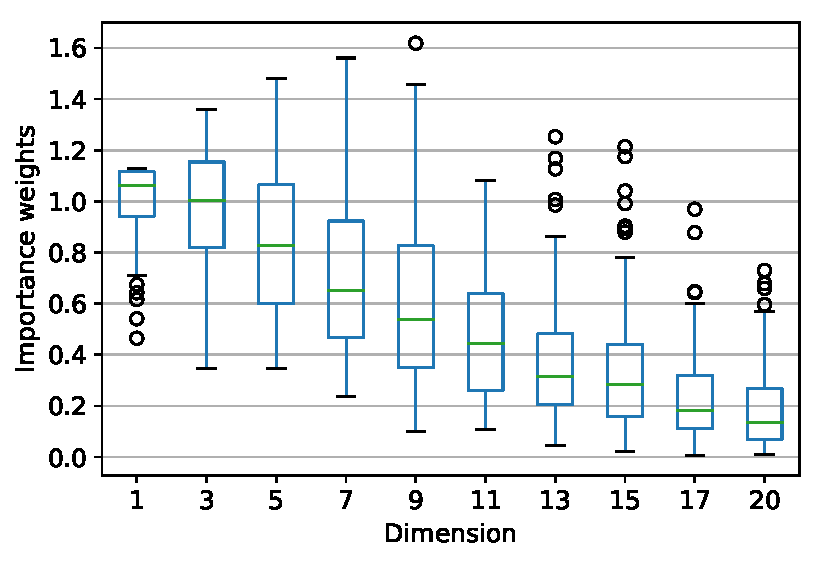
\includegraphics[height=5.1cm]{graphics/importance_mixing/importance_weights_boxplot1.pdf}
        \caption{}
        \label{fig: Theory: importance_mixing/importance_weights_boxplot1.pdf}
    \end{subfigure}
    \hfill
    \begin{subfigure}[b]{0.495\textwidth}
        \centering
        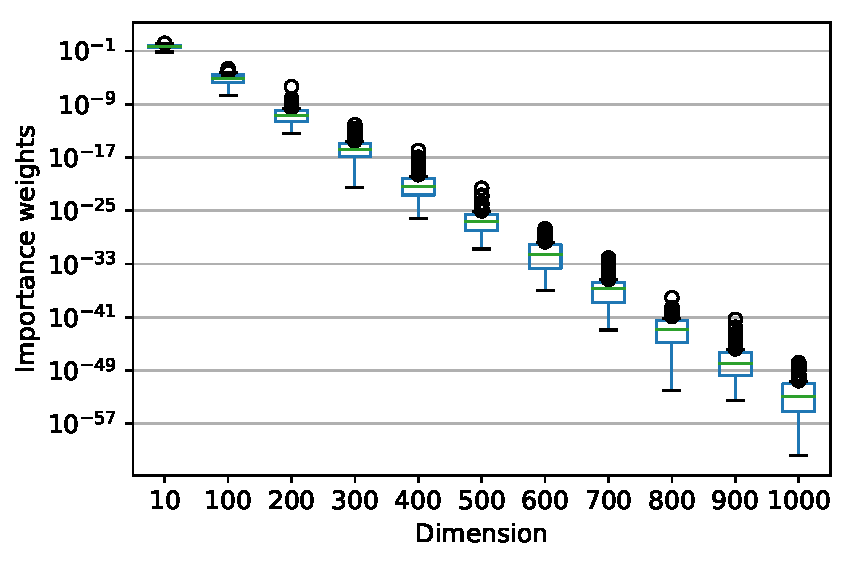
\includegraphics[height=5.1cm]{graphics/importance_mixing/importance_weights_boxplot2.pdf}
        \caption{}
        \label{fig: Theory: importance_mixing/importance_weights_boxplot.pdf2}
    \end{subfigure}
    \caption{Importance weights, such as those used in \autoref{alg: Importance mixing}, collapse for high-dimensional density functions. The figures show boxplots for the distribution of 1000 importance weights computed from samples drawn from a separable Gaussian of different dimensionalities. The importance weights are computed as $\frac{\mathcal{N}(\mub_1+\r,\text{diag}(\sigmab_1+\r)}{\mathcal{N}(\mub_2+\r,\text{diag}(\sigmab_2+\r)}$ with $\mub_1=1.1\e, \sigmab_1=0.9\e, \mub_2=1.0\e, \sigmab_2=1.0\e$ and $\r\sim\mathcal{N}(\0,0.01\e)$. \subref{fig: Theory: importance_mixing/importance_weights_boxplot1.pdf} shows dimensions one to twenty while \subref{fig: Theory: importance_mixing/importance_weights_boxplot.pdf2} shows dimensions up to 1000. (For a reference on interpretation of these boxplots, see \autoref{app: Appendix: Boxplot interpretation}.
    }
    \label{fig: Theory: importance_mixing/importance_weights_boxplot}
\end{figure}


\subsection{Adaptation sampling}\label{sec: Theory: Adaptation sampling}
Adaptation sampling is another probabilistic approach for improving \gls{VO}. As importance mixing, it relies on computation of the importance weights and as such suffers from the curse of dimensionality. Here, it is introduced nevertheless since it can potentially be used to adapt hyperparameters of the optimization problem online including the all-important learning rate. Adaptation sampling has not been used experimentally in this thesis.

First introduced in \cite{Schaul2011a} and further discussed and experimentally validated in \cite{Schaul2012}, adaptation sampling overall works by considering if a fractional change to any certain hyperparameter would have yielded a search distribution more likely to produce the best performing perturbations of the current search distribution. 

This presentation will consider the learning rate applied to the search gradient, $\eta$. Adaptation sampling is then used to determine if a hypothetical search distribution $p(\x|\thetab')$ would have been more likely to generate the best performing samples from the current distribution $p(\x|\thetab)$. The hypothetical distribution is obtained as was the current but by using a slightly larger learning rate $(1+c)\eta$ where $c>0$ is some small number. Then, importance weights are computed in the same way as for importance mixing,
\begin{equation}
    w_i=\frac{p(\x_i|\thetab')}{p(\x_i|\thetab)} \ ,
\end{equation}
for the samples $\x_i\sim p(\x|\thetab)$ for $i=1,\dots,N$. The samples are then ranked based on their fitnesses and being assigned weights with one set of ranks assigned the importance weights while another set gets unit weights,
\begin{equation}
    \begin{aligned}
        S'&\gets\cbra{\pa{w_i,\text{rank}(\x_i)}}\\
        S&\gets\cbra{\pa{1,\text{rank}(\x_i)}} \ .
    \end{aligned}
\end{equation}
The goal is then to decide if $S'$ is superior to $S$. In \cite{Schaul2011a}, a weighted version of the Mann-Whitney test is developed for this purpose. The regular Mann-Whitney test is a non-parametric test of the null hypothesis that it is equally likely that a random sample from the set $S$ will be less than or greater than a random sample from a second set $S'$ \cite{Mann1947}. 
Thus, a rejection of the null hypothesis at significance level $\rho$ is equivalent to concluding that one sample is ``larger" than the other at that significance level. If $S'$ is tested larger than $S$, the learning rate is increased by a fractional amount up to some maximal value $\eta_\text{max}$, 
\begin{equation}
    \eta\gets \min\cbra{(1+c)\eta,\eta_\text{max}}
\end{equation}
where $c$ is some small number. If $S'$ is tested smaller than $S$, the learning rate is decayed towards its initial value,
\begin{equation}
    \eta\gets(1-c)\eta+c\eta_0
\end{equation}
where $\eta_0$ is the initial value. The Mann-Whitney test and its weighted generalization are described in \autoref{app: Weighted Mann-Whitney U-test)} for convenience. The adaptation sampling procedure is summarized in \autoref{alg: Adaptation sampling}.

\begin{algorithm}[tbp!]
    \caption{Adaptation sampling \cite{Schaul2012}. \label{alg: Adaptation sampling}}
    \begin{algorithmic}[1]
        \Require{Search distribution parameters from current and previous iteration, $\thetab_t$ and $\thetab_{t-1}$. Learning rate $\eta$, initial learning rate $\eta_0$ and maximum learning rate $\eta_\text{max}$. Set of samples and associated fitnesses $\{\x_i, f(\x_i)\}$.  Increase factor/decay rate $c$ and significance level $\rho$.}
        \State Compute the hypothetical parameters $\thetab'$ using $(1+c)\eta$.
        \For{each sample $i=1,\dots,N$}
            \State Compute the importance weight 
            $$w_i=\frac{p(\x_i)|\thetab')}{p(\x_i)|\thetab)}$$
        \EndFor
        \State Compute the rank of each sample from its fitness $\{\text{rank}(\x_i)\}$
        \State Let $S$ and $S'$ be the respectively unit weighted and importance weighted sequences of ranks
        $$S\gets\{1,\text{rank}(\x_i)\}$$
        $$S'\gets\{w_i,\text{rank}(\x_i)\}$$
        \State Perform a statistical test to determine if the sequence $S'$ is superior to its $S$.
        \If{$S'$ superior} \Return $\min\cbra{(1+c)\eta, \eta_{\text{max}}}$  \Comment{Increase learning rate}
        \Else{} \Return $(1-c)\eta + c\eta_0$  \Comment{Decay learning rate towards $\eta_0$}
        \EndIf
    \end{algorithmic}
\end{algorithm}

%Although it was shown to improve performance on most of the low-dimensional common black-box optimization bench marks \cite{Schaul2012}, adaptation sampling suffers from the curse of dimensionality and importance weight collapse in the same way as importance mixing. 

% Applications of importance mixing to training of neural networks \cite{Zhao2014}, \cite{Alain2015}, \cite{Katharopoulos2017}, \cite{Katharopoulos2018}



\subsection{Safe mutation}
When perturbing network weights in order to obtain a potentially better performing network there is a significant risk that the learned transformations are broken. This can result in a model that no longer performs anywhere near the performance of the unperturbed model, at worst completely erasing all learned transformations from input to output.

In \cite{Lehman2017a}, a method for coping with this challenge was presented. The publication was part of a series of articles \cite{Lehman2017, Conti2017, Zhang2017, Such2017} that explore optimization of \glspl{NN} in the parameter space by a variant of \gls{VO} based on \cite{Salimans2017}. 
In \cite{Lehman2017a}, backpropagation is used to compute sensitivities of model output units to changes in weights. This sensitivity information can then be used to scale random perturbations of network weights so as to avoid perturbing the model in a manner that changes its output too much.

This section introduces the background of the so-called ``safe mutation" and how to appropriately compute the sensitivities and scale the sampled perturbations based on \cite{Lehman2017a}.


\subsubsection{Output divergence from weight perturbation}
Let $\y(\x,\w)=NN(\x|\w)$ denote the output $\y$ of a neural network $NN$ parameterized by $\w$ and evaluated on some input $\x$. For a mini-batch of $I$ inputs $\X=\bmat{\x_1&\dots&\x_I}$ this gives $\Y(\X,\w)=NN(\X|\w)$ with $Y_{ki}=NN(X_{:,i}|\w)_k$ equal to the $k$'th output unit's value for the $i$'th batch example. 
Now, the divergence of the output of the model that results from an additive perturbation $\epsilonb$ to its weights can be computed by 
\begin{align}
    D(\epsilonb|\w) &=
    \frac{1}{I}\sum_{k=1}^K\sum_{i=1}^I \pa{NN(\x_i|\w)_k - NN(\x_i|\w+\epsilonb)_k}^2\\
    &=
    \frac{1}{I}\sum_{k=1}^K\sum_{i=1}^I \pa{NN(\X|\w)_{ki} - NN(\X|\w+\epsilonb)_{ki}}^2 \ .
    \label{eq: Theory: Variational Optimization - Safe mutation divergence definition}
\end{align}
The divergence can thus be computed by forward propagating a mini-batch through the unperturbed and perturbed networks and summing the element-wise squared differences of their outputs, finally normalizing by the mini-batch size.




\subsubsection{Safe mutation through rescaling (SM-R)}
The simplest way to constrain the divergence of network outputs is to decompose the perturbation into a direction and a magnitude. The direction is sampled from the search distribution but is normalized to have $\norm{\epsilonb}=1$ and is then rescaled to match some predefined amount of divergence. The safe perturbation is then given by
\begin{equation}
    \epsilonb_{\text{safe}} = \alpha\epsilonb \ , 
\end{equation}
where $\alpha>0$ is the magnitude of the rescaling. This magnitude can be found using a simple line search algorithm, requiring a forward pass of the mini-batch in each of the networks and an evaluation of the divergence at every iteration. The mini-batch need not be resampled for this purpose, i.e. in reinforcement learning, no additional rollouts are required if the experiences are stored.

This rescaling approach is appealing due to its well-defined metric of ``safety" that is, it specifically chooses perturbations to give a certain amount of divergence in the network outputs. However, if a few parameters have very high sensitivities, perturbation of these may dominate the divergence and result in a rescaling factor that is very small. In turn, this leads to safe perturbations that are close to zero effectively resulting in the perturbed and unperturbed models being almost identical, $NN(\cdot|\w)\sim NN(\cdot|\w+\epsilonb_\text{safe})$. Geometrically, this is due to the direction of the perturbation being fixed while only the magnitude is rescaled.

While this rescaling approach can be applied to non-differentiable networks, gradient information of the network outputs w.r.t. the weights can be used to also change the direction of the perturbation.


\subsubsection{Safe mutation through gradients (SM-G)}
In order to scale the perturbation direction as well as the magnitude to achieve some reduction in the divergence of the network outputs, the gradient of the network outputs w.r.t. the weights can be computed. As such, safe mutation through gradients can be seen as stopping one step short in the application of the chain rule to the computational graph of the model. Instead of computing the gradient of some objective w.r.t. the network weights, the gradient is computed for the outputs themselves. For instance, in 
\begin{equation}
    \pderiv[1,1]{E}{\w} = \pderiv[1,1]{E}{\y}\pderiv[1,1]{\y}{\w}
\end{equation}
$\pderiv[1,1]{\y}{\w}$ is computed rather than $\pderiv[1,1]{E}{\w}$. In fact, $\pderiv[1,1]{\y}{\w}$ can be seen as being the Jacobian matrix describing the sensitivities of the output units to changes in the weights.

By a first order Taylor expansion, the network output at a single unit $k$ for a single example $\x_i$, $Y_{ki}=NN(\x_{i}|\w)_k$, can be seen as a function of the weight perturbation,
\begin{equation}
    Y_{ki}(\x_i,\epsilonb|\w) \approx NN(\x_{i}|\w)_k + \epsilonb\nabla_\w NN(\x_{i}|\w)_k \ .
\end{equation}
The gradient of the output w.r.t. any weight, $\nabla_\w NN(\x_{i}|\w)_k$, can thus be seen as a single point estimate of the sensitivity of that output unit to that weight. For a mini-batch of inputs, these estimates can be summed and averaged to give a better sensitivity estimate. The sensitivity of the $k$'th output unit can then be written as
\begin{equation*}
     \frac{1}{I}\sum_{i=1}^I \size{\nabla_\w NN(\X|\w)_{ki}} \ .
\end{equation*}
Here it is important to note that to compute this single unit sensitivity, each batch example must be forward propagated, have its loss evaluated, be backpropagated to compute gradients and then the gradients must be replaced by their absolute value. Although the forward pass can be batched, the \emph{absolute} gradients must be accumulated over the mini-batch when backpropagating. All modern numerical libraries for deep learning are designed to efficiently propagate batches of inputs and accumulate \emph{signed} gradients. Accumulating the absolute gradients therefore requires backpropagating each example by itself and computing the absolute gradient before backpropagating the next example. This is rather inefficient.

A much more efficient way to obtain a sensitivity estimate, is to compute an approximate per unit sensitivity by instead simply summing the signed gradients
\begin{equation*}
     \sum_{i=1}^I \nabla_\w NN(\X|\w)_{ki} \ .
\end{equation*}
According to \cite{Lehman2017a}, it empirically improves performance to not average the summed signed gradient over the batch, i.e. not divide by $I$. Summing the signed gradient introduces gradient washout while not dividing by $I$ helps keep the gradient magnitude larger, counteracting the washout.

Since the output layer generally has more than a single unit, i.e. it is a vector contrary to the usual scalar valued error function, both of these two sensitivity estimates result in a gradient for each weight, for each output unit. That is, $K$ gradients are obtained for each weight. To handle this, the gradient from each output unit is interpreted as a component of a $K$-dimensional gradient vector and the total gradient, i.e. the sensitivity, is computed as the Euclidean length of this vector. This results in two variants of the safe mutation,
\begin{align}
    \s_\text{abs} &= \sqrt{\sum_{k=1}^K \pa{\frac{1}{I}\sum_{i=1}^I\size{\nabla_\w NN(\X|\w)_{ki}}}^2}\\
    \s_\text{sum} &= \sqrt{\sum_{k=1}^K \pa{\sum_{i=1}^I\nabla_\w NN(\X|\w)_{ki}}^2} \ .
\end{align}
The absolute gradient variant is computationally much more expensive than the signed gradient variant due to the reasons discussed above. Finally, the sampled perturbation is adjusted to be safe according to the computed sensitivities,
\begin{equation}\label{eq: Theory: Safe mutation scaling}
    \epsilonb_\text{safe} = \frac{\epsilonb}{\s} \ .
\end{equation}


\subsubsection{Safe mutation through Hessian of divergence}
A slightly different approach is to consider the gradient of the divergence defined in \eqref{eq: Theory: Variational Optimization - Safe mutation divergence definition}. This allows perturbing the weights in a way that results in a certain amount of divergence, as in the rescaling approach, but here based on gradients which introduces changes to the direction as well as scaling the magnitude.

However, there is a small catch. The gradient of the divergence can be written as
\begin{align}
    \nabla_\w D(\epsilonb|\w)
    &=
    \frac{1}{I}\nabla_\w\sum_{k=1}^K\sum_{i=1}^I \pa{NN(\X|\w)_{ki} - NN(\X|\w+\epsilonb)_{ki}}^2\nonumber\\
    &=
    \frac{1}{I}\sum_{k=1}^K\sum_{i=1}^I \nabla_\w\pa{NN(\X|\w)_{ki} - NN(\X|\w+\epsilonb)_{ki}}^2\nonumber \ .
    % &=
    % \frac{2}{I}\sum_{k=1}^K\sum_{i=1}^I \pa{NN(\X|\w)_{ki} - NN(\X|\w+\epsilonb)_{ki}}\nabla_\w\pa{NN(\X|\w)_{ki} - NN(\X|\w+\epsilonb)_{ki}}\nonumber
    %&=
    %\frac{2}{I}\sum_{k=1}^K \pa{NN(\X|\w)_{:,k} - NN(\X|\w+\epsilonb)_{:,k}}\pa{\nabla_\w NN(\X|\w)_{:,k} - \nabla_\w NN(\X|\w+\epsilonb)_{:,k}}
\end{align}
% where
% \begin{equation}
%     \nabla_\w\pa{NN(\X|\w)_{ki} - NN(\X|\w+\epsilonb)_{ki}}^2 = 2\pa{NN(\X|\w)_{ki} - NN(\X|\w+\epsilonb)_{ki}}\nabla_\w\pa{NN(\X|\w)_{ki} - NN(\X|\w+\epsilonb)_{ki}}.
% \end{equation}
By the chain rule, the term in the sum becomes
\begin{equation}
    2\pa{NN(\X|\w)_{ki} - NN(\X|\w+\epsilonb)_{ki}}\nabla_\w\pa{NN(\X|\w)_{ki} - NN(\X|\w+\epsilonb)_{ki}} \ .
\end{equation}
When the gradient of the divergence is evaluated at the network's current weights $\epsilonb=0$ this term is zero and as a result, the gradient is zero. Therefore, a second order approximation must be used.

A Taylor expansion of the gradient of the divergence about the current network's weights gives a second order approximation by
\begin{align}
    \nabla_\w D(0+\epsilonb_0|\w)
    &\approx \nabla_\w D(0|\w) + \nabla_\w \bra{ \nabla_\w D(0|\w)\transpose\epsilonb_0} \nonumber\\
    &= 0 + \nabla_\w \bra{\nabla_\w D(0|\w)\transpose}\epsilonb_0 \nonumber\\
    &= \H_\w D(0|\w) \epsilonb_0
\end{align}
% which reduces to
% \begin{equation}
%     \nabla_\w D(0+\epsilonb_0|\w) \approx \H_\w D(0|\w) \epsilonb_0
% \end{equation}
since the gradient of the divergence at $\epsilonb=0$ is zero everywhere\footnote{\label{footnote: Discussion on Hessian versus vector Laplacian}There can be some confusion about the Hessian and the Laplacian. The Hessian operator can be defined as the \textit{outer} product of the gradient operator (nabla) $$\H_\w=\nabla_\w\nabla_\w\transpose$$ while the Laplacian can be defined as the \textit{inner} product of the gradient operator $$\nabla^2_\w=\nabla_\w\transpose\nabla_\w.$$ While the Hessian contains all possible second order partial derivatives, the Laplacian is the trace of the Hessian; a scalar sum of unmixed second order partial derivatives. Here, the Hessian is the operator that arises.}.
Note that the Hessian only needs to be computed as part of a matrix-vector product, $\H_\w D(0|\w) \epsilonb_0$, effectively giving the curvature of the divergence in the direction of the perturbation.

The resulting sensitivities are then computed similarly to before,
\begin{equation}
    \s_\text{SO} = \sqrt{\size{\H_\w D(0|\w)}\epsilonb}
\end{equation}
for an unscaled perturbation $\epsilonb$ which is then adjusted by $\s_\text{SO}$ according to \eqref{eq: Theory: Safe mutation scaling}.


\subsubsection{Numerical considerations}
The computation of the sensitivities derived above requires some consideration to be put into the numerical properties. Both $\s_\text{abs}$ and $\s_\text{sum}$ are computed using at least one non-normalized sum which runs the risk of numerical overflow. The implementation of the sensitivity computation used here sets any sensitivity which has overflowed to $1$. This results in that sensitivity not influencing the perturbation and the perturbation being applied as sampled. Another perhaps more sensible approach would be to set the perturbation to zero and not change the highly sensitive parameter at all. This however risks freezing that parameter indefinitely if the sensitivity does not change considerably. The sensitivity overflow problem occurs extremely rarely.

Another issue is that the numerical value of the sensitivities is somewhat arbitrary. This is most the case with the signed gradient variant which approximates the absolute gradient variant, but the problem also exists for the absolute gradient variant since the $K$ sensitivity gradients are summed at every weight. A normalization can be applied to scale the sensitivities into the range $[0,1]$
\begin{equation}
    % \hat{\s} = \frac{\s-\s_\text{min}}{\s_\text{max} - \s_\text{min}}.
    \hat{\s} = \frac{\s-\min\cbra{\s}}{\max\cbra{\s} - \min\cbra{\s}} \ .
\end{equation}
which is a natural range for a scaling applied by division.
It does however, not remove the risk of the sensitivities being zero or very close to zero which results in very large perturbations. This problem has been handled by clamping the sensitivities below by a small constant,
\begin{equation}
    \hat{\s} \leftarrow \min\cbra{\xi,\hat{\s}}
\end{equation}
Throughout this thesis, the smallest allowed sensitivity has been $\xi=10^{-2}$ which has been found to yield stable rescaling. 

Obtaining $\epsilonb_\text{safe}$ by rescaling with sensitivities in the range $[10^{-2},1]$ does not change the mean of the perturbation since it is zero but it does change the variance. In order to decouple safe mutation from the variance of the perturbation, the perturbation is finally divided by its new variance and multiplied by the wanted variance to get back the original variance in a way that corresponds to the representation and dimensionality of the search distribution. None of these considerations were described in \cite{Lehman2017a}.
